% ============================================================================
% MotorMeasure Pro — Development Journey & Architecture Document
% LaTeX version — compile with pdflatex or xelatex
% ============================================================================
\documentclass[12pt,a4paper]{article}

% ── Packages ────────────────────────────────────────────────────────────────
\usepackage[utf8]{inputenc}
\usepackage[T1]{fontenc}
\usepackage{lmodern}
\usepackage[margin=2.5cm]{geometry}
\usepackage{graphicx}
\usepackage{xcolor}
\usepackage{hyperref}
\usepackage{booktabs}
\usepackage{longtable}
\usepackage{tabularx}
\usepackage{listings}
\usepackage{enumitem}
\usepackage{tikz}
\usepackage{fancyhdr}
\usepackage{titlesec}
\usepackage{tcolorbox}
\usepackage{multicol}
\usepackage{float}
\usepackage{caption}
\usepackage{array}
\usepackage{pgfgantt}
\usepackage{forest}
\usetikzlibrary{shapes.geometric, arrows.meta, positioning, fit, backgrounds, calc}

% ── Colors ──────────────────────────────────────────────────────────────────
\definecolor{primaryteal}{HTML}{0D9488}
\definecolor{darkbg}{HTML}{0F172A}
\definecolor{lightbg}{HTML}{F8FAFC}
\definecolor{codebg}{HTML}{F1F5F9}
\definecolor{sqlblue}{HTML}{1976D2}
\definecolor{linkblue}{HTML}{2563EB}
\definecolor{phase1}{HTML}{3B82F6}
\definecolor{phase2}{HTML}{8B5CF6}
\definecolor{phase3}{HTML}{10B981}
\definecolor{phase4}{HTML}{F59E0B}
\definecolor{phase5}{HTML}{EF4444}

% ── Hyperref setup ──────────────────────────────────────────────────────────
\hypersetup{
    colorlinks=true,
    linkcolor=linkblue,
    urlcolor=linkblue,
    citecolor=linkblue,
    pdftitle={MotorMeasure Pro — Development Journey},
    pdfauthor={Uttkarsh Singh},
}

% ── Code listing style ──────────────────────────────────────────────────────
\lstset{
    backgroundcolor=\color{codebg},
    basicstyle=\ttfamily\small,
    breaklines=true,
    frame=single,
    rulecolor=\color{gray!40},
    tabsize=4,
    showstringspaces=false,
    captionpos=b,
}

\lstdefinestyle{sql}{
    language=SQL,
    keywordstyle=\color{sqlblue}\bfseries,
    commentstyle=\color{gray},
    stringstyle=\color{primaryteal},
}

% ── tcolorbox styles ───────────────────────────────────────────────────────
\tcbuselibrary{skins, breakable}

\newtcolorbox{infobox}[1][]{
    colback=primaryteal!5,
    colframe=primaryteal,
    fonttitle=\bfseries,
    title=#1,
    breakable,
    arc=2mm,
}

\newtcolorbox{quotebox}{
    colback=gray!5,
    colframe=gray!50,
    leftrule=4pt,
    rightrule=0pt,
    toprule=0pt,
    bottomrule=0pt,
    breakable,
    arc=0mm,
}

% ── Header / Footer ────────────────────────────────────────────────────────
\pagestyle{fancy}
\fancyhf{}
\fancyhead[L]{\textcolor{gray}{\small MotorMeasure Pro — Development Journey}}
\fancyhead[R]{\textcolor{gray}{\small \thepage}}
\fancyfoot[C]{\textcolor{gray!60}{\footnotesize GMFM\_System88}}
\renewcommand{\headrulewidth}{0.4pt}

% ── Section styling ────────────────────────────────────────────────────────
\titleformat{\section}
  {\Large\bfseries\color{darkbg}}
  {\thesection.}{0.5em}{}
  [\vspace{-0.5em}\textcolor{primaryteal}{\rule{\textwidth}{1.5pt}}]

\titleformat{\subsection}
  {\large\bfseries\color{darkbg}}
  {\thesubsection}{0.5em}{}

\titleformat{\subsubsection}
  {\normalsize\bfseries\color{darkbg}}
  {\thesubsubsection}{0.5em}{}

% ── Column type for tables ─────────────────────────────────────────────────
\newcolumntype{L}[1]{>{\raggedright\arraybackslash}p{#1}}
\newcolumntype{C}[1]{>{\centering\arraybackslash}p{#1}}

% ============================================================================
\begin{document}

% ── Title Page ──────────────────────────────────────────────────────────────
\begin{titlepage}
\centering
\vspace*{3cm}

{\Huge\bfseries\textcolor{darkbg}{MotorMeasure Pro}}\\[0.5cm]
{\Large\textcolor{primaryteal}{Development Journey \& Architecture Document}}\\[2cm]

\textcolor{primaryteal}{\rule{0.6\textwidth}{2pt}}\\[1.5cm]

\begin{tabular}{rl}
    \textbf{Project:}     & GMFM\_System88 / MotorMeasure Pro \\[0.3cm]
    \textbf{Period:}      & November 2025 -- March 2026 \\[0.3cm]
    \textbf{Author:}      & Uttkarsh Singh \\[0.3cm]
    \textbf{Codebase:}    & $\sim$34 source files, $\sim$1.4\,MB of code \\[0.3cm]
    \textbf{Version:}     & 0.0.3 \\
\end{tabular}

\vfill
{\small\textcolor{gray}{Generated on March 30, 2026}}
\end{titlepage}

% ── Table of Contents ───────────────────────────────────────────────────────
\tableofcontents
\newpage

% ============================================================================
\section{What Is This Project?}
% ============================================================================

\textbf{MotorMeasure Pro} is a \textbf{cross-platform clinical assessment application} that digitizes the \textbf{Gross Motor Function Measure (GMFM-88)} scoring process. The GMFM is a standardized tool used by physiotherapists and clinicians to measure gross motor function in children with cerebral palsy and other motor disabilities.

The app replaces paper-based scoresheets with a mobile-first digital workflow, enabling clinicians to:

\begin{itemize}[leftmargin=2em]
    \item \textbf{Score all 88 items} across 5 motor domains (0--3 scale + Not Tested)
    \item \textbf{Manage student/patient profiles} with encrypted personal data
    \item \textbf{Track progress over time} with session history and trend charts
    \item \textbf{Generate PDF reports} that match the official GMFM scoresheet format
    \item \textbf{Sync data to the cloud} via Supabase for backup and multi-device access
\end{itemize}

% ============================================================================
\section{Technology Stack}
% ============================================================================

\begin{table}[H]
\centering
\renewcommand{\arraystretch}{1.3}
\begin{tabularx}{\textwidth}{l l X}
\toprule
\textbf{Layer} & \textbf{Technology} & \textbf{Purpose} \\
\midrule
Language         & Python 3.11+                          & Core runtime \\
UI Framework     & Flet 0.28.3                           & Cross-platform UI (Flutter-based, renders natively) \\
Local Database   & SQLite (via \texttt{sqlite3})          & Offline-first persistence \\
Cloud Backend    & Supabase (PostgreSQL + Auth)           & Cloud sync, user authentication \\
PDF Generation   & fpdf2 / ReportLab / Raw PDF            & Clinical report generation (triple fallback) \\
Charts           & Matplotlib (optional)                  & Trend visualization \\
Data Validation  & Pydantic (with dataclass fallback)     & Model validation \\
Encryption       & \texttt{cryptography} (Fernet)         & Field-level encryption at rest \\
Password Hashing & PBKDF2-SHA256 (200k iterations)        & Secure local authentication \\
DOCX Import      & python-docx                            & Import existing assessments \\
Build Target     & Flet CLI (\texttt{flet build apk/ipa}) & Android APK / iOS builds \\
\bottomrule
\end{tabularx}
\caption{Technology stack overview}
\end{table}

\subsection{Key Design Decision: Triple PDF Fallback}

The report service implements a \textbf{3-tier fallback} for PDF generation:

\begin{enumerate}
    \item \textbf{ReportLab} --- Full-featured (desktop, needs C extensions)
    \item \textbf{fpdf2} --- Pure Python (works on Android)
    \item \textbf{Raw PDF} --- Zero dependencies, hand-crafted PDF byte stream ($\sim$300 lines of raw PDF operators)
\end{enumerate}

This ensures reports work on \emph{every} platform, even when no PDF library is available.

% ============================================================================
\section{Git Commit History \& Development Timeline}
% ============================================================================

\begin{quotebox}
\texttt{23 commits over $\sim$4 months by Uttkarsh Singh}
\end{quotebox}

\begin{longtable}{c l l l l}
\toprule
\textbf{\#} & \textbf{Date} & \textbf{Commit} & \textbf{Message} & \textbf{Phase} \\
\midrule
\endhead
1  & 2025-11-17 & \texttt{375251d} & Initial commit               & \textcolor{phase1}{Foundation} \\
2  & 2025-11-22 & \texttt{edeff63} & some\_updates                & \textcolor{phase1}{Foundation} \\
3  & 2025-11-22 & \texttt{2f050de} & ui\_changes                  & \textcolor{phase2}{UI} \\
4  & 2025-11-28 & \texttt{6da6253} & some\_changes                & \textcolor{phase1}{Iteration} \\
5  & 2025-12-07 & \texttt{b3be147} & new flet                     & \textcolor{phase2}{Framework Upgrade} \\
6  & 2025-12-07 & \texttt{48f6984} & changes                      & \textcolor{phase1}{Iteration} \\
7  & 2025-12-08 & \texttt{061acaa} & ui\_improvements             & \textcolor{phase2}{UI Polish} \\
8  & 2025-12-08 & \texttt{fbc7656} & del                          & \textcolor{gray}{Cleanup} \\
9  & 2025-12-08 & \texttt{d0535d7} & ando                         & \textcolor{phase3}{Android} \\
10 & 2025-12-09 & \texttt{0d8e6c3} & needs to be fixed            & \textcolor{phase5}{Bug Fix} \\
11 & 2025-12-10 & \texttt{8763df8} & haptics                      & \textcolor{phase3}{Haptic Feedback} \\
12 & 2026-01-05 & \texttt{8a530c2} & changes\_to\_add\_DOCX       & \textcolor{phase3}{DOCX Import} \\
13 & 2026-01-12 & \texttt{0a97b29} & changes                      & \textcolor{phase1}{Iteration} \\
14 & 2026-01-12 & \texttt{a576dd5} & ignores                      & \textcolor{gray}{Git Config} \\
15 & 2026-01-24 & \texttt{3b42538} & Update instructions\_data.json & \textcolor{phase3}{Content} \\
16 & 2026-02-28 & \texttt{6123f95} & uodate\_yeah                 & \textcolor{phase1}{Update} \\
17 & 2026-03-02 & \texttt{0e16d4b} & android\_fixed               & \textcolor{phase4}{Android Fix} \\
18 & 2026-03-02 & \texttt{9544430} & android\_fixed               & \textcolor{phase4}{Android Fix} \\
19 & 2026-03-02 & \texttt{71e6877} & optimised                    & \textcolor{phase4}{Optimization} \\
20 & 2026-03-02 & \texttt{dcb9b47} & final?                       & \textcolor{phase4}{Stabilization} \\
21 & 2026-03-02 & \texttt{cfeed0e} & logo\_added                  & \textcolor{phase2}{Branding} \\
22 & 2026-03-02 & \texttt{942e0c8} & things\_done                 & \textcolor{phase4}{Stabilization} \\
23 & 2026-03-16 & \texttt{483cd11} & 0.0.3, login                 & \textcolor{phase5}{Auth System} \\
\bottomrule
\end{longtable}

\subsection{Development Phases (Gantt Chart)}

\begin{figure}[H]
\centering
\begin{ganttchart}[
    hgrid,
    vgrid={*{6}{draw=gray!30}},
    x unit=0.35cm,
    y unit chart=0.6cm,
    title height=1,
    bar height=0.5,
    bar top shift=0.25,
    title label font=\footnotesize,
    bar label font=\footnotesize,
    group label font=\footnotesize\bfseries,
    milestone label font=\footnotesize,
    time slot format=isodate,
    time slot unit=day,
]{2025-11-15}{2026-03-20}

    \gantttitlecalendar{year, month} \\

    \ganttbar[bar/.style={fill=phase1}]{Foundation}{2025-11-17}{2025-11-28} \\
    \ganttbar[bar/.style={fill=phase2}]{UI \& Framework}{2025-12-07}{2025-12-10} \\
    \ganttbar[bar/.style={fill=phase3}]{Features}{2026-01-05}{2026-01-24} \\
    \ganttbar[bar/.style={fill=phase4}]{Hardening}{2026-02-28}{2026-03-02} \\
    \ganttbar[bar/.style={fill=phase5}]{Auth \& Sync}{2026-03-02}{2026-03-16}

\end{ganttchart}
\caption{MotorMeasure Pro Development Timeline}
\end{figure}

% ============================================================================
\section{Architecture Overview}
% ============================================================================

\subsection{Layered Architecture Diagram}

\begin{figure}[H]
\centering
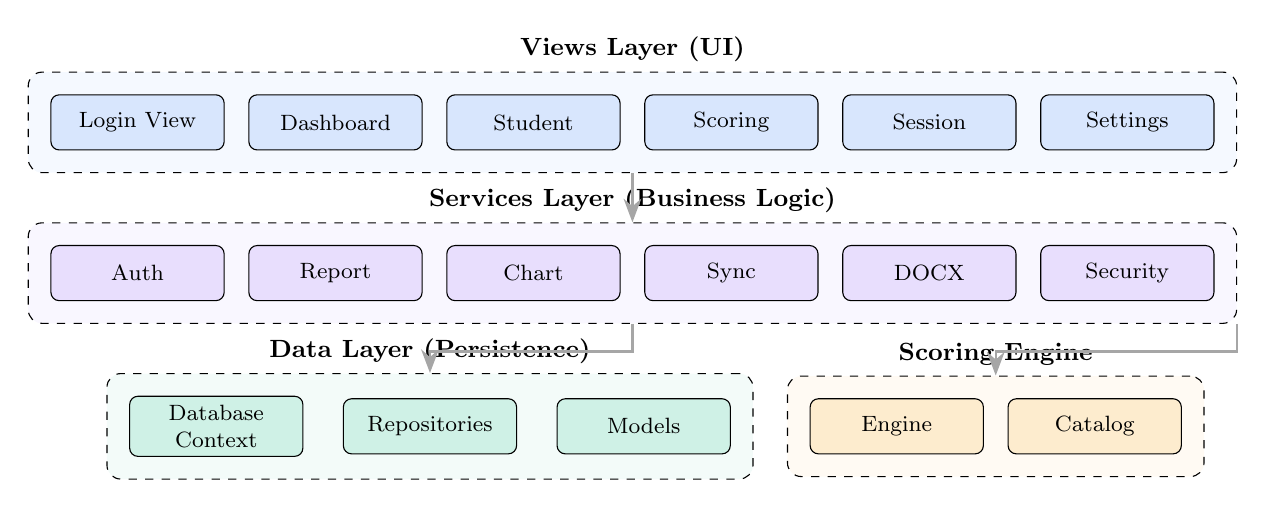
\begin{tikzpicture}[
    node distance=0.4cm,
    box/.style={draw, rounded corners=3pt, minimum width=2.2cm, minimum height=0.7cm, font=\footnotesize, align=center},
    layer/.style={draw, dashed, rounded corners=5pt, inner sep=8pt, fill=#1!5},
    arrow/.style={-{Stealth[length=3mm]}, thick, draw=gray!70},
]

% Views layer
\node[box, fill=phase1!20] (lv) {Login View};
\node[box, fill=phase1!20, right=0.3cm of lv] (dv) {Dashboard};
\node[box, fill=phase1!20, right=0.3cm of dv] (stv) {Student};
\node[box, fill=phase1!20, right=0.3cm of stv] (sv) {Scoring};
\node[box, fill=phase1!20, right=0.3cm of sv] (sev) {Session};
\node[box, fill=phase1!20, right=0.3cm of sev] (setv) {Settings};

\begin{scope}[on background layer]
\node[layer=phase1, fit=(lv)(setv), label={[font=\small\bfseries]above:Views Layer (UI)}] (views) {};
\end{scope}

% Services layer
\node[box, fill=phase2!20, below=1.2cm of lv] (as) {Auth};
\node[box, fill=phase2!20, right=0.3cm of as] (rs) {Report};
\node[box, fill=phase2!20, right=0.3cm of rs] (cs) {Chart};
\node[box, fill=phase2!20, right=0.3cm of cs] (ss) {Sync};
\node[box, fill=phase2!20, right=0.3cm of ss] (ds) {DOCX};
\node[box, fill=phase2!20, right=0.3cm of ds] (hs) {Security};

\begin{scope}[on background layer]
\node[layer=phase2, fit=(as)(hs), label={[font=\small\bfseries]above:Services Layer (Business Logic)}] (services) {};
\end{scope}

% Data layer
\node[box, fill=phase3!20, below=1.2cm of as, xshift=1cm] (db) {Database\\Context};
\node[box, fill=phase3!20, right=0.5cm of db] (rp) {Repositories};
\node[box, fill=phase3!20, right=0.5cm of rp] (md) {Models};

\begin{scope}[on background layer]
\node[layer=phase3, fit=(db)(md), label={[font=\small\bfseries]above:Data Layer (Persistence)}] (data) {};
\end{scope}

% Scoring engine
\node[box, fill=phase4!20, right=1cm of md] (en) {Engine};
\node[box, fill=phase4!20, right=0.3cm of en] (ct) {Catalog};

\begin{scope}[on background layer]
\node[layer=phase4, fit=(en)(ct), label={[font=\small\bfseries]above:Scoring Engine}] (scoring) {};
\end{scope}

% Arrows
\draw[arrow] (views.south) -- ++(0,-0.35) -| (services.north);
\draw[arrow] (services.south) -- ++(0,-0.35) -| (data.north);
\draw[arrow] (services.south east) -- ++(0,-0.35) -| (scoring.north);

\end{tikzpicture}
\caption{Layered application architecture}
\end{figure}

\subsection{Module Breakdown}

\subsubsection{\texttt{src/gmfm\_app/main.py} --- Application Entry Point (600 lines)}

\begin{itemize}[leftmargin=2em]
    \item \textbf{GMFMApp class} --- Core app controller with views-based routing
    \item \textbf{Splash screen} --- Animated logo sequence with fade transitions
    \item \textbf{Platform detection} --- Auto-detects Android/iOS vs desktop
    \item \textbf{Theme management} --- Dark/Light mode with persistence
    \item \textbf{Route management} --- Custom URL-based navigation with history stack
    \item \textbf{Navigation locking} --- Prevents concurrent nav (fixes blank-screen bugs)
    \item \textbf{Background DB init} --- Database loads in a separate thread during splash
\end{itemize}

\subsubsection{\texttt{src/gmfm\_app/data/} --- Data Layer}

\begin{table}[H]
\centering
\renewcommand{\arraystretch}{1.3}
\begin{tabularx}{\textwidth}{l c X}
\toprule
\textbf{File} & \textbf{Lines} & \textbf{Purpose} \\
\midrule
\texttt{database.py}     & 220 & SQLite connection factory, 8 schema migrations, multi-platform path resolution \\
\texttt{models.py}       & 107 & \texttt{Student}, \texttt{Session}, \texttt{AppUser} --- Pydantic with dataclass fallback \\
\texttt{repositories.py} & 370 & CRUD operations with per-user data isolation, sync queue logging \\
\bottomrule
\end{tabularx}
\caption{Data layer modules}
\end{table}

\textbf{Key patterns:}
\begin{itemize}[leftmargin=2em]
    \item \textbf{Dual model system} --- Uses Pydantic if available, falls back to dataclasses (for Android compatibility)
    \item \textbf{Per-user data isolation} --- All queries filter by \texttt{user\_id} when available
    \item \textbf{Sync queue} --- Every write operation logs to \texttt{sync\_queue} table for offline-first cloud sync
    \item \textbf{Encrypted fields} --- Patient names and identifiers encrypted using Fernet before storage
\end{itemize}

\subsubsection{\texttt{src/gmfm\_app/scoring/} --- GMFM-88 Scoring Engine}

\begin{table}[H]
\centering
\renewcommand{\arraystretch}{1.3}
\begin{tabularx}{\textwidth}{l c X}
\toprule
\textbf{File} & \textbf{Lines} & \textbf{Purpose} \\
\midrule
\texttt{engine.py}         & 77    & Domain percentage calculation, total score computation \\
\texttt{constants.py}      & 55    & Lazy-loaded \texttt{\_LazyItems} class for GMFM-88 item mappings \\
\texttt{items\_catalog.py} & $\sim$100 & Item number $\rightarrow$ domain mapping builder, domain metadata \\
\texttt{items\_data.json}  & ---   & All 88 GMFM items with numbers, descriptions, and domains \\
\bottomrule
\end{tabularx}
\caption{Scoring engine modules}
\end{table}

\textbf{Scoring algorithm:}
\begin{itemize}[leftmargin=2em]
    \item Maps 88 items across 5 domains: A (Lying \& Rolling), B (Sitting), C (Crawling \& Kneeling), D (Standing), E (Walking \& Running)
    \item Each item scored 0--3 or NT (Not Tested)
    \item Per-domain percentage $= \dfrac{\text{sum of scored items}}{\text{count} \times 3} \times 100$
    \item Total percentage = weighted average across all domains
\end{itemize}

\subsubsection{\texttt{src/gmfm\_app/services/} --- Business Logic Layer}

\begin{table}[H]
\centering
\renewcommand{\arraystretch}{1.3}
\begin{tabularx}{\textwidth}{l c X}
\toprule
\textbf{File} & \textbf{Lines} & \textbf{Purpose} \\
\midrule
\texttt{auth\_service.py}        & 179 & Local auth (PBKDF2-SHA256) + auto cloud login via Supabase \\
\texttt{sync\_service.py}        & 402 & Offline-first sync engine: push/pull/sync with Supabase \\
\texttt{sync\_worker.py}         & 85  & Background thread auto-syncing every 60s \\
\texttt{sync\_config.py}         & 60  & Supabase connection config, stored in Flet client\_storage \\
\texttt{report\_service.py}      & 644 & Triple PDF fallback (ReportLab $\rightarrow$ fpdf2 $\rightarrow$ raw PDF) \\
\texttt{chart\_service.py}       & 94  & Matplotlib trend charts (total + per-domain) \\
\texttt{docx\_import\_service.py} & 324 & Parse GMFM DOCX files, extract multi-session assessments \\
\texttt{security.py}             & 92  & Fernet encryption, key resolution (env $\rightarrow$ file $\rightarrow$ generate) \\
\texttt{haptics.py}              & 82  & Haptic feedback patterns (optimized for Nothing Phone 2a) \\
\texttt{instructions\_service.py} & 100 & Load exercise instructions from JSON (multi-path Android compat) \\
\texttt{ui\_scale.py}            & 125 & Android accessibility scaling (reads system text\_scale\_factor) \\
\texttt{instructions\_data.json} & --- & 80\,KB of exercise instructions (scoring criteria, descriptions) \\
\bottomrule
\end{tabularx}
\caption{Services layer modules}
\end{table}

\subsubsection{\texttt{src/gmfm\_app/views/} --- UI Layer}

\begin{table}[H]
\centering
\renewcommand{\arraystretch}{1.3}
\begin{tabularx}{\textwidth}{l c X}
\toprule
\textbf{File} & \textbf{Lines} & \textbf{Purpose} \\
\midrule
\texttt{login\_view.py}     & $\sim$370 & Login + registration, first admin setup, form validation \\
\texttt{dashboard\_view.py} & $\sim$640 & Student cards, stats, recent sessions, search, quick actions \\
\texttt{student\_view.py}   & $\sim$250 & Add/edit student profiles (name, DOB, identifier) \\
\texttt{scoring\_view.py}   & $\sim$690 & Scoring interface --- all 88 items across 5 domains with in-app instructions \\
\texttt{session\_view.py}   & $\sim$760 & Session history, detail view, session comparison \\
\texttt{settings\_view.py}  & $\sim$645 & Cloud sync config, theme toggle, DOCX import, data management \\
\bottomrule
\end{tabularx}
\caption{UI layer modules}
\end{table}

% ============================================================================
\section{Database Schema}
% ============================================================================

\subsection{Local SQLite Schema}

\begin{lstlisting}[style=sql, caption={Local SQLite schema}]
-- Core tables
students    (id, given_name*, family_name*, dob, identifier*,
             created_at, user_id)
sessions    (id, student_id, scale, raw_scores, total_score,
             notes, created_at, user_id)
app_users   (id, username, password_hash, full_name, role,
             is_active, email, created_at)
settings    (key, value)

-- Sync infrastructure
sync_queue    (id, table_name, record_id, operation, payload,
               created_at, synced)
sync_metadata (key, value)

-- * = Fernet-encrypted at rest
\end{lstlisting}

\subsection{Cloud Schema (Supabase PostgreSQL)}

\begin{lstlisting}[style=sql, caption={Supabase cloud schema}]
students  (id, user_id, local_id, given_name, family_name,
           dob, identifier, deleted, created_at, updated_at)
sessions  (id, user_id, local_id, student_local_id, scale,
           raw_scores, total_score, deleted, created_at, updated_at)
sync_metadata (id, user_id, key, value)

-- Row Level Security: each user can only see their own data
-- Indexes on user_id for performance
\end{lstlisting}

\subsection{Schema Migrations}

The app handles 8 in-code migrations:

\begin{enumerate}
    \item Rename \texttt{patients} $\rightarrow$ \texttt{students} table
    \item Add \texttt{notes} column to sessions
    \item Add \texttt{role} and \texttt{is\_active} to app\_users
    \item Rename \texttt{patient\_id} $\rightarrow$ \texttt{student\_id} in sessions
    \item Add \texttt{email} column to app\_users
    \item Add \texttt{user\_id} to students (data isolation)
    \item Add \texttt{user\_id} to sessions (data isolation)
    \item Create \texttt{sync\_queue} and \texttt{sync\_metadata} tables
\end{enumerate}

% ============================================================================
\section{Key Feature Deep-Dives}
% ============================================================================

\subsection{Offline-First Cloud Sync}

The sync system follows a \textbf{git-like model}:

\begin{figure}[H]
\centering
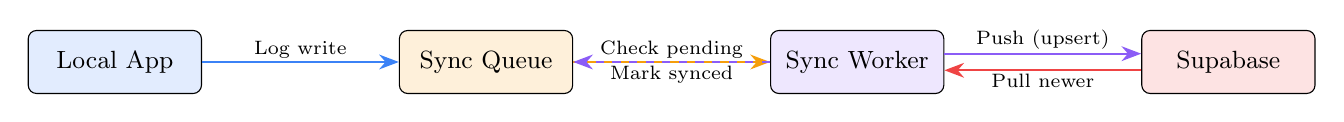
\begin{tikzpicture}[
    entity/.style={draw, rounded corners=3pt, minimum width=2.2cm, minimum height=0.8cm, font=\small, align=center, fill=#1!15},
    msg/.style={-{Stealth[length=2.5mm]}, thick, draw=#1},
    msglabel/.style={font=\scriptsize, fill=white, inner sep=1pt},
]

\node[entity=phase1] (app) {Local App};
\node[entity=phase4, right=2.5cm of app] (queue) {Sync Queue};
\node[entity=phase2, right=2.5cm of queue] (worker) {Sync Worker};
\node[entity=phase5, right=2.5cm of worker] (cloud) {Supabase};

% Arrows
\draw[msg=phase1] (app) -- node[msglabel, above] {Log write} (queue);
\draw[msg=phase4] (queue) -- node[msglabel, above] {Check pending} (worker);
\draw[msg=phase2] ([yshift=3pt]worker.east) -- node[msglabel, above] {Push (upsert)} ([yshift=3pt]cloud.west);
\draw[msg=phase5] ([yshift=-3pt]cloud.west) -- node[msglabel, below] {Pull newer} ([yshift=-3pt]worker.east);
\draw[msg=phase2, dashed] (worker) -- node[msglabel, below] {Mark synced} (queue);

\end{tikzpicture}
\caption{Offline-first sync data flow}
\end{figure}

\begin{itemize}[leftmargin=2em]
    \item \textbf{Local wins}: Pending local changes skip cloud pull for the same record
    \item \textbf{Soft deletes}: Cloud uses \texttt{deleted} flag instead of hard delete
    \item \textbf{Auto-retry}: Background worker retries every 60 seconds
    \item \textbf{Connectivity check}: Pings \texttt{8.8.8.8:53} before attempting sync
\end{itemize}

\subsection{Authentication System}

Two-tier authentication:

\begin{enumerate}
    \item \textbf{Local}: PBKDF2-SHA256 with 200,000 iterations, 16-byte random salt
    \item \textbf{Cloud}: Auto-registers/logs-in to Supabase Auth when email is provided
\end{enumerate}

Session is stored in Flet's \texttt{client\_storage} (persists across app restarts). All routes except \texttt{/login} are protected.

\subsection{PDF Report Generation}

Generates clinical-grade GMFM scoresheets with:

\begin{itemize}[leftmargin=2em]
    \item Student information header
    \item Total score banner (teal branded)
    \item Domain summary table (5 domains + totals)
    \item Detailed item-by-item score tables (88 items with 0/1/2/3/NT marks)
    \item Notes section
    \item Optional trend chart embedding
\end{itemize}

The \textbf{raw PDF fallback} ($\sim$300 lines) hand-crafts the PDF binary format including:

\begin{itemize}[leftmargin=2em]
    \item Custom \texttt{\_PdfPage} class with graphics/text streams
    \item Bordered table cells with fill colors
    \item Multi-page support with automatic page breaks
    \item Proper xref table and trailer construction
\end{itemize}

\subsection{Android Compatibility Layer}

Special handling for mobile deployment:

\begin{itemize}[leftmargin=2em]
    \item \texttt{FLET\_APP\_STORAGE\_DATA} env var for private storage paths
    \item Embedded base64 splash assets (logos in \texttt{splash\_assets.py} --- 1\,MB)
    \item Lazy imports to avoid crashing when libraries aren't available
    \item Multi-path file resolution for JSON data files
    \item Android accessibility scaling (reads \texttt{text\_scale\_factor})
    \item Haptic feedback optimized for Nothing Phone 2a's linear motor
\end{itemize}

% ============================================================================
\section{Development Journey Narrative}
% ============================================================================

\subsection{Phase 1: Foundation (Nov 17--28, 2025)}

The project started with the \textbf{Initial commit} on November 17, 2025. The early architecture document references \textbf{KivyMD} as the UI toolkit, indicating the app was originally designed with Kivy before being ported to Flet. The initial setup included:

\begin{itemize}[leftmargin=2em]
    \item Core database schema (\texttt{patients} $\rightarrow$ later renamed to \texttt{students})
    \item Basic GMFM-88 scoring engine
    \item Pydantic models for data validation
    \item SQLite persistence layer
\end{itemize}

Two follow-up commits in late November refined the UI and added foundational changes.

\subsection{Phase 2: Framework Migration \& UI Polish (Dec 7--10, 2025)}

A critical pivot occurred in early December: the commit \textbf{``new flet''} (\texttt{b3be147}) signals the \textbf{migration from KivyMD to Flet}. This was likely driven by Flet's superior cross-platform capabilities and easier Android deployment. Over 3 intense days:

\begin{itemize}[leftmargin=2em]
    \item UI was rebuilt with Flet components
    \item Android builds were attempted (commit \texttt{d0535d7}: ``ando'')
    \item Issues emerged (``needs to be fixed'')
    \item \textbf{Haptic feedback} was added, specifically optimized for the Nothing Phone 2a
    \item UI cleanup and improvements were made across multiple commits
\end{itemize}

\subsection{Phase 3: Feature Expansion (Jan 5 -- Jan 24, 2026)}

After a holiday break, January brought significant feature additions:

\begin{itemize}[leftmargin=2em]
    \item \textbf{DOCX Import Service} --- Parse existing GMFM assessment documents (supporting multi-session files with multiple date headers)
    \item \textbf{Exercise Instructions} --- 80\,KB JSON database of all 88 exercise descriptions, scoring criteria, starting positions, and instructions
    \item \textbf{.gitignore refinements} to keep the repository clean
\end{itemize}

\subsection{Phase 4: Stabilization \& Android Fixes (Feb 28 -- Mar 2, 2026)}

A major push in late February / early March focused on making the Android build reliable:

\begin{itemize}[leftmargin=2em]
    \item Multiple \textbf{Android-specific fixes} (path resolution, import errors, asset loading)
    \item \textbf{Performance optimization} pass
    \item \textbf{Logo and branding} integration (base64-embedded splash assets)
    \item Multiple commits in a single day (Mar 2: 6 commits) showing rapid iteration and testing
\end{itemize}

\subsection{Phase 5: Authentication \& Cloud Sync (Mar 2--16, 2026)}

The final phase added enterprise-grade features:

\begin{itemize}[leftmargin=2em]
    \item \textbf{Local authentication} with secure password hashing (PBKDF2-SHA256)
    \item \textbf{User registration and login} views
    \item \textbf{Per-user data isolation} --- each user only sees their own students/sessions
    \item \textbf{Supabase cloud backend} integration with Row Level Security
    \item \textbf{Offline-first sync engine} following a git-like push/pull model
    \item \textbf{Background sync worker} running on a 60-second interval
    \item Version tagged as \textbf{v0.0.3}
\end{itemize}

% ============================================================================
\section{File \& Code Statistics}
% ============================================================================

\begin{table}[H]
\centering
\renewcommand{\arraystretch}{1.4}
\begin{tabular}{l r}
\toprule
\textbf{Metric} & \textbf{Value} \\
\midrule
Total source files (\texttt{.py} + \texttt{.json})  & 34 \\
Total source code size                                & $\sim$1.4\,MB \\
Largest file                                          & \texttt{splash\_assets.py} ($\sim$1\,MB) \\
Total \texttt{.py} lines (excluding assets)           & $\sim$5,500+ \\
Git commits                                           & 23 \\
Development period                                    & 4 months \\
Views                                                 & 6 \\
Services                                              & 12 \\
Database tables                                       & 6 \\
Schema migrations                                     & 8 \\
GMFM items scored                                     & 88 \\
Motor domains                                         & 5 \\
\bottomrule
\end{tabular}
\caption{Codebase statistics}
\end{table}

% ============================================================================
\section{Project Files at a Glance}
% ============================================================================

\begin{lstlisting}[basicstyle=\ttfamily\scriptsize, frame=none, backgroundcolor=\color{codebg}]
GMFM_System88/
|-- src/
|   |-- main.py                          # Outer entry point
|   |-- entry_point.py                   # Android entry point
|   |-- requirements.txt                 # flet, fpdf2, supabase
|   +-- gmfm_app/
|       |-- main.py                      # App bootstrap (600 lines)
|       |-- main_desktop.py              # Desktop-specific launcher
|       |-- splash_assets.py             # Base64-encoded logos (~1 MB)
|       |-- data/
|       |   |-- database.py              # SQLite + migrations
|       |   |-- models.py                # Pydantic/dataclass models
|       |   +-- repositories.py          # CRUD + sync queue
|       |-- scoring/
|       |   |-- engine.py                # GMFM-88 scoring algorithm
|       |   |-- constants.py             # Lazy-loaded item mappings
|       |   |-- items_catalog.py         # Domain/item builder
|       |   +-- items_data.json          # All 88 items catalog
|       |-- services/
|       |   |-- auth_service.py          # PBKDF2 local auth + cloud
|       |   |-- sync_service.py          # Push/pull sync engine
|       |   |-- sync_worker.py           # Background auto-sync
|       |   |-- sync_config.py           # Supabase config management
|       |   |-- report_service.py        # 3-tier PDF generation
|       |   |-- chart_service.py         # Matplotlib trend charts
|       |   |-- docx_import_service.py   # DOCX assessment parser
|       |   |-- security.py              # Fernet encryption provider
|       |   |-- haptics.py               # Mobile haptic feedback
|       |   |-- instructions_service.py  # Exercise instructions loader
|       |   |-- instructions_data.json   # 88 exercise descriptions
|       |   +-- ui_scale.py              # Android accessibility scale
|       +-- views/
|           |-- login_view.py            # Auth UI
|           |-- dashboard_view.py        # Main dashboard
|           |-- student_view.py          # Student profile form
|           |-- scoring_view.py          # GMFM scoring interface
|           |-- session_view.py          # History + detail + compare
|           +-- settings_view.py         # Settings + sync + import
|-- docs/
|   |-- architecture.md                  # Architecture documentation
|   +-- gmfm_scoresheet.txt              # Reference scoresheet
|-- tests/
|   |-- test_scoring.py                  # Scoring engine tests
|   +-- test_docx_import_verify.py       # DOCX parser tests
|-- supabase_schema.sql                  # Cloud database schema + RLS
|-- README.md                            # Project documentation
|-- GMFCS.docx                           # Reference GMFCS document
|-- gmfm-88_and_66_scoresheet.pdf        # Official GMFM scoresheet
|-- architecture_diagram.png             # Architecture diagram
|-- workflow_diagram.png                 # Workflow diagram
|-- problem_diagram.png                  # Problem statement diagram
|-- GMFM_Presentation.pptx              # Project presentations
|-- GMFM_Pro_Presentation.pptx
+-- MotorMeasure_Pro_Presentation.pptx
\end{lstlisting}

% ============================================================================
\section{Roadmap}
% ============================================================================

Future planned features (from README):

\begin{itemize}[leftmargin=2em]
    \item[$\square$] Remote sync adapter for multi-device support
    \item[$\square$] Role-based access control for clinical teams
    \item[$\square$] GMFCS classification integration
    \item[$\square$] Automated deployment packages
    \item[$\square$] GMFM-66 scale-specific calculations (item difficulty lookup tables)
    \item[$\square$] CLI export tool (\texttt{python -m gmfm\_app.cli export})
\end{itemize}

% ============================================================================
\end{document}
